%-----------------------------------
\newcommand{\meta}[2]{
	\begin{frame}
		\frametitle{#1}
		\centering
		{\fontsize{5cm}{1em}\selectfont \textbf{#2}}
	\end{frame}
}
%-----------------------------------


\section{Metacaracteres}
\frame{\tableofcontents[currentsection]}

\subsection{Caracteres e Metacaracteres}

\begin{frame}
	\frametitle{Você sabe o que são os metacaracteres?}
	
	\begin{itemize}
		\item Se você não conhecia essas belezinhas de \textit{expressões regulares} você só utilizou caracteres literais durante toda sua vida;

		\item Metacaracteres, você, você metacaracteres;

		\item Como isso vai fazer diferença na minha vida?

		\item Diferença dos robozinhos.		
	\end{itemize}
\end{frame}

\begin{frame}
	\begin{figure}
		\centering
			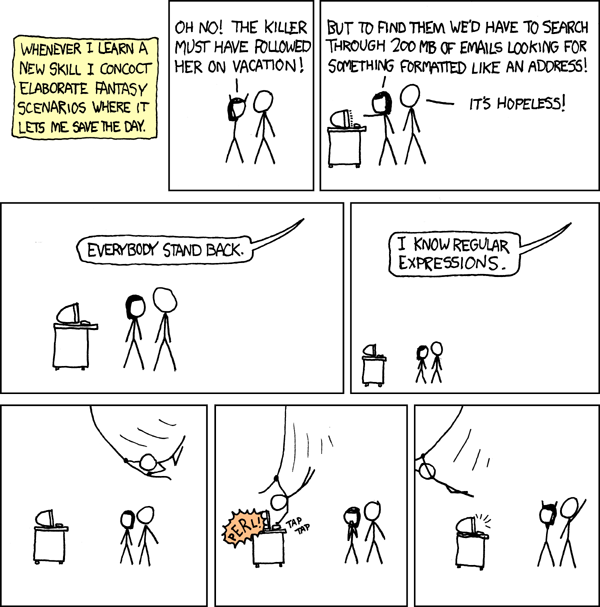
\includegraphics[height=0.8\textheight]{imagens/re/regular_expressions.png}
		\caption{Expressões Regulares salvando o dia}
	\end{figure}

\end{frame}

\begin{frame}
	\frametitle{Tipos}
	\Large{\azul{Representante} e \azul{Quantificador}}
\end{frame}

\subsection{Tipo representante}

%------------------------------------------------
\meta{Ponto}{.}

\begin{frame}
	\frametitle{O ponto}
	\Large{O ponto casa com \azul{TUDO}.}
	
	i.e., o ponto casa com qualquer caractere!

	\azul{Pergunta}: o ponto casa com um ponto?
\end{frame}

\begin{frame}
	\begin{figure}
		\centering
		
\includegraphics[height=0.8\textheight]{./imagens/re/sad_joker.jpeg}
		\caption{O ponto é o coringa solitário.}
	\end{figure}
\end{frame}

\begin{frame}
	\frametitle{Casamento do ponto}
	\begin{center}
		\begin{tabular}{ c | c }
		\textbf{Expressão}	& \textbf{Casa com...}		\\ \hline
		n.o			& nao, não, n40, noo...  	\\ \hline
		.u			& au, bu, du...		 	\\ \hline
		12.45			& 12:45, 12 45, 12.45... 	\\ \hline
		\end{tabular}
	\end{center}

\end{frame}

%------------------------------------------------
\meta{Lista}{[...]}

\begin{frame}
	\frametitle{A lista}
	\begin{itemize}
		\item \Large{A lista casa com \azul{TODOS} os caracteres dentro dela.}
		\item \textbf{Exemplos}: [abc], [123], [letras]...
		\item \large{\bf Dentro da lista todo mundo é LITERAL.}
		\begin{itemize}
			\item O ponto dentro da lista é literal;
		\end{itemize}
	\end{itemize}
\end{frame}

\begin{frame}
	\frametitle{Mentiroso!}
	\begin{itemize}
		\item Lembra que eu falei que todo mundo dentro lista era literal? Então... \Large{\bf EU MENTI \vermelho{MUAHAHAHA}}.
	\end{itemize}
\end{frame}

\begin{frame}
	\frametitle{Mentiroso (nem tanto, vai)!}
	\begin{itemize}
		\item Lembra que eu falei que todo mundo dentro lista era literal? Então...
		\begin{itemize}
			\item Todo caractere que se acha fora da lista, lá dentro não serve pra nada ou tem outro significado;
			\item É como se ela tivesse um mundinho dentro dela, só dela, onde ela dita as regras.
		\end{itemize}
	\end{itemize}
\end{frame}
%------------------------------------------------
\meta{Lista Negada}{[\textasciicircum...]}

\begin{frame}
	\frametitle{A lista negada}
	\begin{itemize}
		\item \Large{A \azul{lista negada} casa com \azul{TODOS} os caracteres que \textbf{\vermelho{NÃO}} estão dentro dela.}
		\item Ou seja, ela não é tão seletiva quanto a lista, tampouco liberal quanto o ponto. Ela sabe com quem não quer casar;
		\item \textbf{Exemplos}: [\textasciicircum abc], [\textasciicircum 123], [\textasciicircum letras]...
	\end{itemize}
\end{frame}

%SOBRE LISTAS--------------------------------------
\begin{frame}
	\frametitle{Intervalos}
	
	\begin{itemize}
		\item Como você faria uma expressão regular para casar com dois números consecutivos?
	\end{itemize}
\end{frame}

\begin{frame}
	\frametitle{Intervalos}
	
	\begin{itemize}
		\item Como você faria uma expressão regular para casar com dois números consecutivos?
		\begin{itemize}
			\item "\textbf{[0123456789][0123456789]}"?
		\end{itemize}
	\end{itemize}
\end{frame}

\begin{frame}
	\frametitle{Intervalos}

	\begin{itemize}
		\item O traço (-) é um operador não literal dentro da lista;
		\item Ele foi criado para representar intervalos:
			\begin{itemize}
				\item \lista{0-9} é igual a \lista{0123456789};
				\item \lista{a-z} é igual a \lista{abcdefghijklmnopqrstuvwxyz};
				\item \lista{A-Z} é igual a \lista{ABCDEFGHIJKLMNOPQRSTUVWXYZ};
				\item \lista{0-9a-zA-Z}
				\item \lista{ -\textasciitilde}
			\end{itemize}
	\end{itemize}
\end{frame}

\begin{frame}
	\frametitle{Intervalos}

	\begin{itemize}
		\item O traço (-) é o único operador não literal dentro da lista;
		\item Ele foi criado para representar intervalos:
			\begin{itemize}
				\item \lista{0-9} é igual a \lista{0123456789};
				\item \lista{a-z} é igual a \lista{abcdefghijklmnopqrstuvwxyz};
				\item \lista{A-Z} é igual a \lista{ABCDEFGHIJKLMNOPQRSTUVWXYZ};
				\item \lista{0-9a-zA-Z};
				\item \lista{ -\textasciitilde}\Huge{\bf \vermelho{???}}
			\end{itemize}
	\end{itemize}
\end{frame}

\begin{frame}
	\frametitle{Exceções}
	
	\begin{itemize}
		\item \textbf{E se eu quiser colocar um traço (-) na lista?}
		\item \textbf{E se eu quiser colocar os colchetes (\lcol  e \rcol) na lista?}
		\item \textbf{E se eu quiser colocar um circunflexo na lista?}
		\item \textbf{E se...}
	\end{itemize}

\end{frame}

\begin{frame}
	\frametitle{Exceções}
	
	\begin{itemize}
		\item \textbf{E se eu quiser colocar um traço (-) na lista?}
		\begin{itemize}
			\item Devemos color o traço no começo ou no final da lista;
			\item \lista{-0-9} $\rightarrow$ Casa com 0 a 9 e traço;
			\item \lista{a-f-} $\rightarrow$ Casa com a a f e traço;
		\end{itemize}
		\item \textbf{E se eu quiser colocar os colchetes (\lcol  e \rcol) na lista?}
		\item \textbf{E se eu quiser colocar um circunflexo na lista?}
		\item \textbf{E se...}
	\end{itemize}

\end{frame}

\begin{frame}
	\frametitle{Exceções}
	
	\begin{itemize}
		\item \textbf{E se eu quiser colocar um traço (-) na lista?}
		\item \textbf{E se eu quiser colocar os colchetes (\lcol  e \rcol) na lista?}
		\begin{itemize}
			\item O "colchete abrir" podemos colocar em qualquer lugar:
			\begin{itemize}
				\item \lista{\lcol0-9};
				\item \lista{0-4\lcol*.ç};
			\end{itemize}
			\item O "colchete de fechar" deve ser o primeiro da lista;
			\begin{itemize}
				\item \lista{\rcol0-9} $\rightarrow$ Casa com 0 a 9 ou com \rcol.
				\item \lista{0-9\rcol} $\rightarrow$ Tá errado.
			\end{itemize}
		\end{itemize}
		\item \textbf{E se eu quiser colocar um circunflexo na lista?}
		\item \textbf{E se...}
	\end{itemize}

\end{frame}

\begin{frame}
	\frametitle{Exceções}
	
	\begin{itemize}
		\item \textbf{E se eu quiser colocar um traço (-) na lista?}
		\item \textbf{E se eu quiser colocar os colchetes (\lcol  e \rcol) na lista?}
		\item \textbf{E se eu quiser colocar um circunflexo na lista?}
			\begin{itemize}
				\item \lista{a-z\textasciicircum}$\rightarrow$casa com caracteres de a a z e \textasciicircum;
				\item \lista{\textasciicircum a-z}$\rightarrow$lista negada: casa com qualquer coisa que não seja de a a z.
			\end{itemize}
		\item \textbf{E se...}
	\end{itemize}

\end{frame}

\begin{frame}
	\frametitle{Exceções}
	
	\begin{itemize}
		\item \textbf{E se eu quiser colocar um traço (-) na lista?}
		\item \textbf{E se eu quiser colocar os colchetes (\lcol  e \rcol) na lista?}
		\item \textbf{E se eu quiser colocar um circunflexo na lista?}
		\item \textbf{E se...}
		\begin{itemize}
			\item Mais alguma coisa/dúvida?
		\end{itemize}
	\end{itemize}

\end{frame}

\begin{frame}
	\frametitle{Casamento das listas}
	\begin{center}
	\begin{tabular}{ c | c }
		\textbf{Expressão} & \textbf{Casa com...} \\ \hline
		n[aãAÃ]o	&	nao, não, nAo, nÃo \\ \hline
		12[:. ]45	&	12:45, 12.45, 12 45 \\ \hline
		funcao.[ch]	&	funcao.c, funcao.h   \\ \hline
		[][-]		&	\textbf{???}		\\ \hline

	\end{tabular}
	\end{center}
\end{frame}

\begin{frame}
	\frametitle{Casamento das listas}
	\begin{center}
	\begin{tabular}{ c | c }
		\textbf{Expressão} & \textbf{Casa com...} \\ \hline
		n[aãAÃ]o	&	nao, não, nAo, nÃo \\ \hline
		12[:. ]45	&	12:45, 12.45, 12 45 \\ \hline
		funcao.[ch]	&	funcao.c, funcao.h   \\ \hline
		[][-]		&	[, ], -		\\ \hline
	\end{tabular}
	\end{center}
\end{frame}

%------------------------------------------------
\subsection{Tipo Quantificador}

%------------------------------------------------
\meta{Opcional}{?}

%------------------------------------------------
\meta{Asterisco}{*}

%------------------------------------------------
\meta{Mais}{+}

%------------------------------------------------
\meta{Chaves}{ \{m,n\} }

%------------------------------------------------
\subsection{Tipo Âncora}

%------------------------------------------------
\meta{Circunflexo}{\textasciicircum}

%------------------------------------------------
\meta{Cifrão}{\$}

%------------------------------------------------
\meta{Borda}{\textbackslash b}

%------------------------------------------------
\subsection{Outros}

%------------------------------------------------
\meta{Ou}{|}

%------------------------------------------------
\meta{Escape}{\textbackslash n}

%------------------------------------------------
\meta{Grupo}{(...)}

%------------------------------------------------
\meta{Retrovisor}{\textbackslash 1...\textbackslash 9}
